\chapter{Programming Languages}

Programming languages are different levels of binary abstraction, the ones and zeroes that make up the computer's language. Commands to the computer are written in a particular language and then compiled into binary.
These compilers are different for each language. Each language also has a different garbage collection form, redundant data handling, and other specifics. Therefore, each language has certain specialities and operates at different speeds.
We make a distinction between high level and low-level languages. High-level languages compile automatically at runtime and have built-in garbage collection. Some low-level languages require developers to handle garbage collection themselves and compile their code into an executable file before running it.
That makes lower-level languages more customisable and, as a result, often faster.
Therefore, we consider low-level languages like C++ and Rust to be faster for most use-cases, and higher-level languages like Python and JavaScript are considered slower.
In this thesis, C++, a low-level language and Python, a high-level language, are pitted against each other to explore what difference the choice of language makes on the same application in terms of speed and energy efficiency.

\section{C++}
C++ is based on the traditional C language. We consider C++ a low-level language because it lacks automatic memory management. Many different compilers are available for C++, making it a portable language. "C++ compiles directly to a machine's native code, allowing it to be one of the fastest languages in the world if optimised" \cite{C++}.
For the research in this thesis, an Apple MacBook computer was used. The Operating System (OS) is macOS Monterey, which ships with the C++ compiler clang, as seen in figure 3.1. “The Clang project provides a language front-end and tooling infrastructure for languages in the C language family (C, C++, Objective C/C++, OpenCL, CUDA, and RenderScript) for the LLVM project” \cite{clang}. Clang is also used in production to build software like Chrome or Firefox. The clang compiler is incorporated into the macOS native Xcode IDE (integrated development environment), which was used for the research in this thesis.

\begin{figure}[htbp]
	\centering
	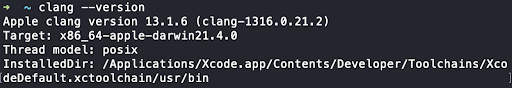
\includegraphics[scale=0.72]{clang.png}
	\caption{clang version on MacBook Pro}
	\label{figure:clang}
\end{figure}

\section{Python}
Python is an open-source, interpreted, object-oriented programming language. "It incorporates modules, exceptions, dynamic typing, very high-level dynamic data types, and classes." It runs on many operating systems like macOS, Windows and Linux.
The language comes with a sizeable standard library for many different purposes. For example, Python is often used for experimenting and logging, string processing and internet protocols like HTTP. Besides the standard library, there is also a wide variety of third-party extensions available \cite{python}.
